\documentclass[11pt, oneside]{article}   	% use "amsart" instead of "article" for AMSLaTeX format
\usepackage{geometry}                		% See geometry.pdf to learn the layout options. There are lots.
\usepackage{textcomp}
\usepackage{hyperref}  % TODO: see page 94 of latex book
\geometry{letterpaper}                   		% ... or a4paper or a5paper or ... 
%\usepackage[parfill]{parskip}    		% Activate to begin paragraphs with an empty line rather than an indent
\usepackage{graphicx}				% Use pdf, png, jpg, or eps§ with pdflatex; use eps in DVI mode
								% TeX will automatically convert eps --> pdf in pdflatex		
\usepackage{amssymb}
\usepackage{relsize}

\title{CSCI 181 / E-181 Spring 2014 Practical 2 \\ 
{\large Kaggle Team "No Comment"}
}
\author{
  David Wihl\\
  \texttt{davidwihl@gmail.com}
  \and
  Zack Hendlin\\
  \texttt{zgh@mit.edu} 
}
%\date{}							% Activate to display a given date or no date

\begin{document}
\maketitle
\section*{Warm-Up}

%max g-forces eyeballs out is 12g eyeballs out http://www.gforces.net/human-tolerance-horizontal.html

%helmet tests on g forces http://www.smf.org/docs/articles/hic/Various_helmets_stds.pdf

\subsection*{Baseline}

\begin{figure}[h!] 
  \centering
  \scalebox{0.5}{{\large % GNUPLOT: LaTeX picture with Postscript
\begingroup
  \makeatletter
  \providecommand\color[2][]{%
    \GenericError{(gnuplot) \space\space\space\@spaces}{%
      Package color not loaded in conjunction with
      terminal option `colourtext'%
    }{See the gnuplot documentation for explanation.%
    }{Either use 'blacktext' in gnuplot or load the package
      color.sty in LaTeX.}%
    \renewcommand\color[2][]{}%
  }%
  \providecommand\includegraphics[2][]{%
    \GenericError{(gnuplot) \space\space\space\@spaces}{%
      Package graphicx or graphics not loaded%
    }{See the gnuplot documentation for explanation.%
    }{The gnuplot epslatex terminal needs graphicx.sty or graphics.sty.}%
    \renewcommand\includegraphics[2][]{}%
  }%
  \providecommand\rotatebox[2]{#2}%
  \@ifundefined{ifGPcolor}{%
    \newif\ifGPcolor
    \GPcolorfalse
  }{}%
  \@ifundefined{ifGPblacktext}{%
    \newif\ifGPblacktext
    \GPblacktexttrue
  }{}%
  % define a \g@addto@macro without @ in the name:
  \let\gplgaddtomacro\g@addto@macro
  % define empty templates for all commands taking text:
  \gdef\gplbacktext{}%
  \gdef\gplfronttext{}%
  \makeatother
  \ifGPblacktext
    % no textcolor at all
    \def\colorrgb#1{}%
    \def\colorgray#1{}%
  \else
    % gray or color?
    \ifGPcolor
      \def\colorrgb#1{\color[rgb]{#1}}%
      \def\colorgray#1{\color[gray]{#1}}%
      \expandafter\def\csname LTw\endcsname{\color{white}}%
      \expandafter\def\csname LTb\endcsname{\color{black}}%
      \expandafter\def\csname LTa\endcsname{\color{black}}%
      \expandafter\def\csname LT0\endcsname{\color[rgb]{1,0,0}}%
      \expandafter\def\csname LT1\endcsname{\color[rgb]{0,1,0}}%
      \expandafter\def\csname LT2\endcsname{\color[rgb]{0,0,1}}%
      \expandafter\def\csname LT3\endcsname{\color[rgb]{1,0,1}}%
      \expandafter\def\csname LT4\endcsname{\color[rgb]{0,1,1}}%
      \expandafter\def\csname LT5\endcsname{\color[rgb]{1,1,0}}%
      \expandafter\def\csname LT6\endcsname{\color[rgb]{0,0,0}}%
      \expandafter\def\csname LT7\endcsname{\color[rgb]{1,0.3,0}}%
      \expandafter\def\csname LT8\endcsname{\color[rgb]{0.5,0.5,0.5}}%
    \else
      % gray
      \def\colorrgb#1{\color{black}}%
      \def\colorgray#1{\color[gray]{#1}}%
      \expandafter\def\csname LTw\endcsname{\color{white}}%
      \expandafter\def\csname LTb\endcsname{\color{black}}%
      \expandafter\def\csname LTa\endcsname{\color{black}}%
      \expandafter\def\csname LT0\endcsname{\color{black}}%
      \expandafter\def\csname LT1\endcsname{\color{black}}%
      \expandafter\def\csname LT2\endcsname{\color{black}}%
      \expandafter\def\csname LT3\endcsname{\color{black}}%
      \expandafter\def\csname LT4\endcsname{\color{black}}%
      \expandafter\def\csname LT5\endcsname{\color{black}}%
      \expandafter\def\csname LT6\endcsname{\color{black}}%
      \expandafter\def\csname LT7\endcsname{\color{black}}%
      \expandafter\def\csname LT8\endcsname{\color{black}}%
    \fi
  \fi
  \setlength{\unitlength}{0.0500bp}%
  \begin{picture}(11520.00,8640.00)%
    \gplgaddtomacro\gplbacktext{%
      \colorrgb{0.00,0.00,0.00}%
      \put(860,640){\makebox(0,0)[r]{\strut{}-150}}%
      \colorrgb{0.00,0.00,0.00}%
      \put(860,2120){\makebox(0,0)[r]{\strut{}-100}}%
      \colorrgb{0.00,0.00,0.00}%
      \put(860,3600){\makebox(0,0)[r]{\strut{}-50}}%
      \colorrgb{0.00,0.00,0.00}%
      \put(860,5079){\makebox(0,0)[r]{\strut{}0}}%
      \colorrgb{0.00,0.00,0.00}%
      \put(860,6559){\makebox(0,0)[r]{\strut{}50}}%
      \colorrgb{0.00,0.00,0.00}%
      \put(860,8039){\makebox(0,0)[r]{\strut{}100}}%
      \colorrgb{0.00,0.00,0.00}%
      \put(980,440){\makebox(0,0){\strut{}-10}}%
      \colorrgb{0.00,0.00,0.00}%
      \put(2434,440){\makebox(0,0){\strut{}0}}%
      \colorrgb{0.00,0.00,0.00}%
      \put(3888,440){\makebox(0,0){\strut{}10}}%
      \colorrgb{0.00,0.00,0.00}%
      \put(5342,440){\makebox(0,0){\strut{}20}}%
      \colorrgb{0.00,0.00,0.00}%
      \put(6797,440){\makebox(0,0){\strut{}30}}%
      \colorrgb{0.00,0.00,0.00}%
      \put(8251,440){\makebox(0,0){\strut{}40}}%
      \colorrgb{0.00,0.00,0.00}%
      \put(9705,440){\makebox(0,0){\strut{}50}}%
      \colorrgb{0.00,0.00,0.00}%
      \put(11159,440){\makebox(0,0){\strut{}60}}%
      \colorrgb{0.00,0.00,0.00}%
      \put(160,4339){\rotatebox{90}{\makebox(0,0){\strut{}force on head (g)}}}%
      \colorrgb{0.00,0.00,0.00}%
      \put(6069,140){\makebox(0,0){\strut{}time since impact(ms)}}%
      \csname LTb\endcsname%
      \put(6069,8339){\makebox(0,0){\strut{}Linear Basis}}%
    }%
    \gplgaddtomacro\gplfronttext{%
      \csname LTb\endcsname%
      \put(10256,7876){\makebox(0,0)[r]{\strut{}Training Data}}%
      \csname LTb\endcsname%
      \put(10256,7676){\makebox(0,0)[r]{\strut{}Linear Basis}}%
    }%
    \gplbacktext
    \put(0,0){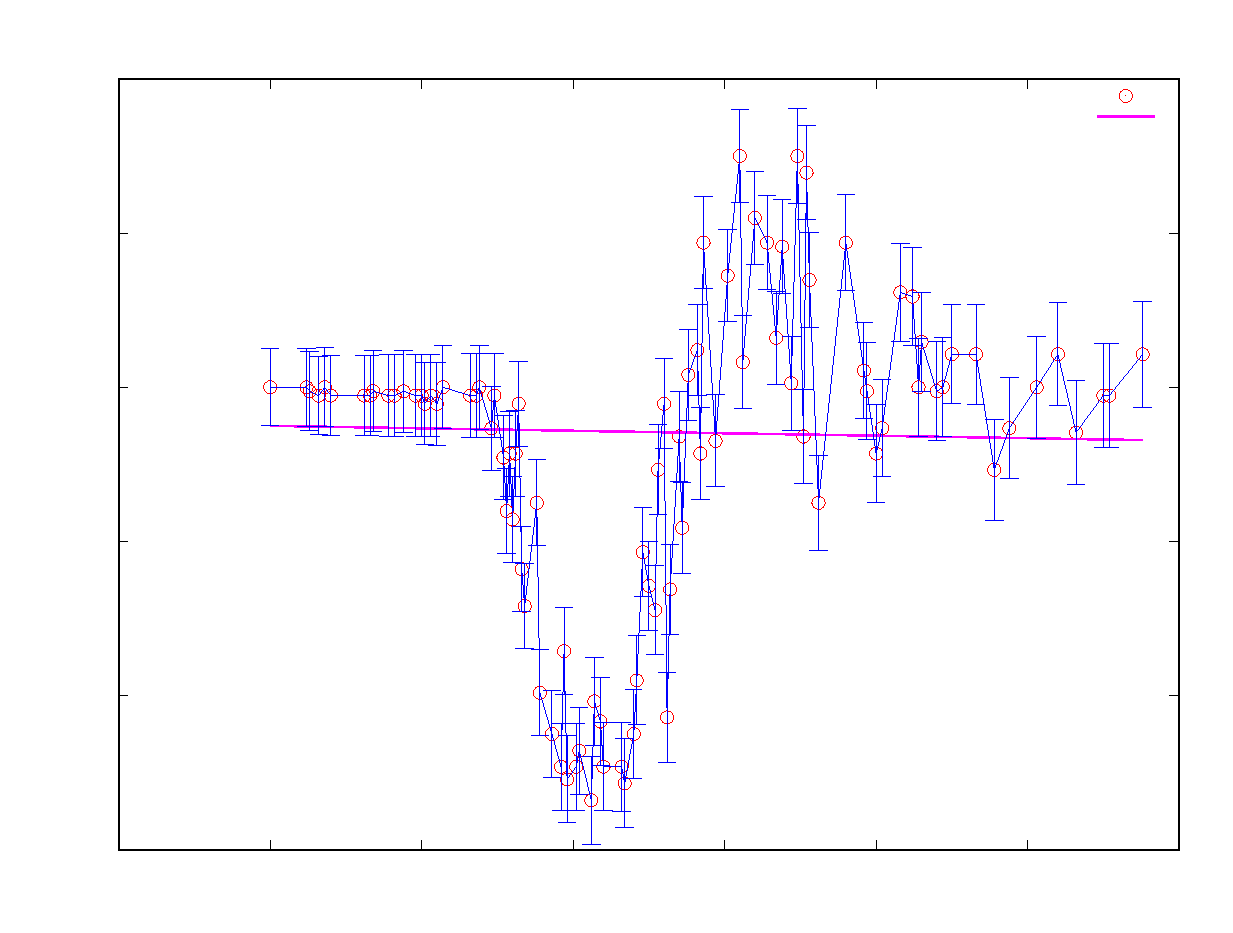
\includegraphics{linear}}%
    \gplfronttext
  \end{picture}%
\endgroup
}}
  \caption{Warmup: Linear Basis}
\end{figure}

As a baseline, we first created a simple linear gradient descent with a flat slope and intercept. 

We also used a polynomial basis, iterating with polynomials from $n^2$ up to $n^{12}$ and selecting the lowest error. Unsurprisingly, $n^{12}$ had the lowest error rate, but is likely highly overfit.

\begin{figure}[h!] 
  \centering
  \scalebox{0.5}{{\large % GNUPLOT: LaTeX picture with Postscript
\begingroup
  \makeatletter
  \providecommand\color[2][]{%
    \GenericError{(gnuplot) \space\space\space\@spaces}{%
      Package color not loaded in conjunction with
      terminal option `colourtext'%
    }{See the gnuplot documentation for explanation.%
    }{Either use 'blacktext' in gnuplot or load the package
      color.sty in LaTeX.}%
    \renewcommand\color[2][]{}%
  }%
  \providecommand\includegraphics[2][]{%
    \GenericError{(gnuplot) \space\space\space\@spaces}{%
      Package graphicx or graphics not loaded%
    }{See the gnuplot documentation for explanation.%
    }{The gnuplot epslatex terminal needs graphicx.sty or graphics.sty.}%
    \renewcommand\includegraphics[2][]{}%
  }%
  \providecommand\rotatebox[2]{#2}%
  \@ifundefined{ifGPcolor}{%
    \newif\ifGPcolor
    \GPcolorfalse
  }{}%
  \@ifundefined{ifGPblacktext}{%
    \newif\ifGPblacktext
    \GPblacktexttrue
  }{}%
  % define a \g@addto@macro without @ in the name:
  \let\gplgaddtomacro\g@addto@macro
  % define empty templates for all commands taking text:
  \gdef\gplbacktext{}%
  \gdef\gplfronttext{}%
  \makeatother
  \ifGPblacktext
    % no textcolor at all
    \def\colorrgb#1{}%
    \def\colorgray#1{}%
  \else
    % gray or color?
    \ifGPcolor
      \def\colorrgb#1{\color[rgb]{#1}}%
      \def\colorgray#1{\color[gray]{#1}}%
      \expandafter\def\csname LTw\endcsname{\color{white}}%
      \expandafter\def\csname LTb\endcsname{\color{black}}%
      \expandafter\def\csname LTa\endcsname{\color{black}}%
      \expandafter\def\csname LT0\endcsname{\color[rgb]{1,0,0}}%
      \expandafter\def\csname LT1\endcsname{\color[rgb]{0,1,0}}%
      \expandafter\def\csname LT2\endcsname{\color[rgb]{0,0,1}}%
      \expandafter\def\csname LT3\endcsname{\color[rgb]{1,0,1}}%
      \expandafter\def\csname LT4\endcsname{\color[rgb]{0,1,1}}%
      \expandafter\def\csname LT5\endcsname{\color[rgb]{1,1,0}}%
      \expandafter\def\csname LT6\endcsname{\color[rgb]{0,0,0}}%
      \expandafter\def\csname LT7\endcsname{\color[rgb]{1,0.3,0}}%
      \expandafter\def\csname LT8\endcsname{\color[rgb]{0.5,0.5,0.5}}%
    \else
      % gray
      \def\colorrgb#1{\color{black}}%
      \def\colorgray#1{\color[gray]{#1}}%
      \expandafter\def\csname LTw\endcsname{\color{white}}%
      \expandafter\def\csname LTb\endcsname{\color{black}}%
      \expandafter\def\csname LTa\endcsname{\color{black}}%
      \expandafter\def\csname LT0\endcsname{\color{black}}%
      \expandafter\def\csname LT1\endcsname{\color{black}}%
      \expandafter\def\csname LT2\endcsname{\color{black}}%
      \expandafter\def\csname LT3\endcsname{\color{black}}%
      \expandafter\def\csname LT4\endcsname{\color{black}}%
      \expandafter\def\csname LT5\endcsname{\color{black}}%
      \expandafter\def\csname LT6\endcsname{\color{black}}%
      \expandafter\def\csname LT7\endcsname{\color{black}}%
      \expandafter\def\csname LT8\endcsname{\color{black}}%
    \fi
  \fi
  \setlength{\unitlength}{0.0500bp}%
  \begin{picture}(11520.00,8640.00)%
    \gplgaddtomacro\gplbacktext{%
      \colorrgb{0.00,0.00,0.00}%
      \put(860,640){\makebox(0,0)[r]{\strut{}-300}}%
      \colorrgb{0.00,0.00,0.00}%
      \put(860,2120){\makebox(0,0)[r]{\strut{}-200}}%
      \colorrgb{0.00,0.00,0.00}%
      \put(860,3600){\makebox(0,0)[r]{\strut{}-100}}%
      \colorrgb{0.00,0.00,0.00}%
      \put(860,5079){\makebox(0,0)[r]{\strut{}0}}%
      \colorrgb{0.00,0.00,0.00}%
      \put(860,6559){\makebox(0,0)[r]{\strut{}100}}%
      \colorrgb{0.00,0.00,0.00}%
      \put(860,8039){\makebox(0,0)[r]{\strut{}200}}%
      \colorrgb{0.00,0.00,0.00}%
      \put(980,440){\makebox(0,0){\strut{}-10}}%
      \colorrgb{0.00,0.00,0.00}%
      \put(2434,440){\makebox(0,0){\strut{}0}}%
      \colorrgb{0.00,0.00,0.00}%
      \put(3888,440){\makebox(0,0){\strut{}10}}%
      \colorrgb{0.00,0.00,0.00}%
      \put(5342,440){\makebox(0,0){\strut{}20}}%
      \colorrgb{0.00,0.00,0.00}%
      \put(6797,440){\makebox(0,0){\strut{}30}}%
      \colorrgb{0.00,0.00,0.00}%
      \put(8251,440){\makebox(0,0){\strut{}40}}%
      \colorrgb{0.00,0.00,0.00}%
      \put(9705,440){\makebox(0,0){\strut{}50}}%
      \colorrgb{0.00,0.00,0.00}%
      \put(11159,440){\makebox(0,0){\strut{}60}}%
      \colorrgb{0.00,0.00,0.00}%
      \put(160,4339){\rotatebox{90}{\makebox(0,0){\strut{}force on head (g)}}}%
      \colorrgb{0.00,0.00,0.00}%
      \put(6069,140){\makebox(0,0){\strut{}time since impact(ms)}}%
      \csname LTb\endcsname%
      \put(6069,8339){\makebox(0,0){\strut{}Polynomial Basis}}%
    }%
    \gplgaddtomacro\gplfronttext{%
      \csname LTb\endcsname%
      \put(10256,7876){\makebox(0,0)[r]{\strut{}Training Data}}%
      \csname LTb\endcsname%
      \put(10256,7676){\makebox(0,0)[r]{\strut{}Polynomial Basis}}%
    }%
    \gplbacktext
    \put(0,0){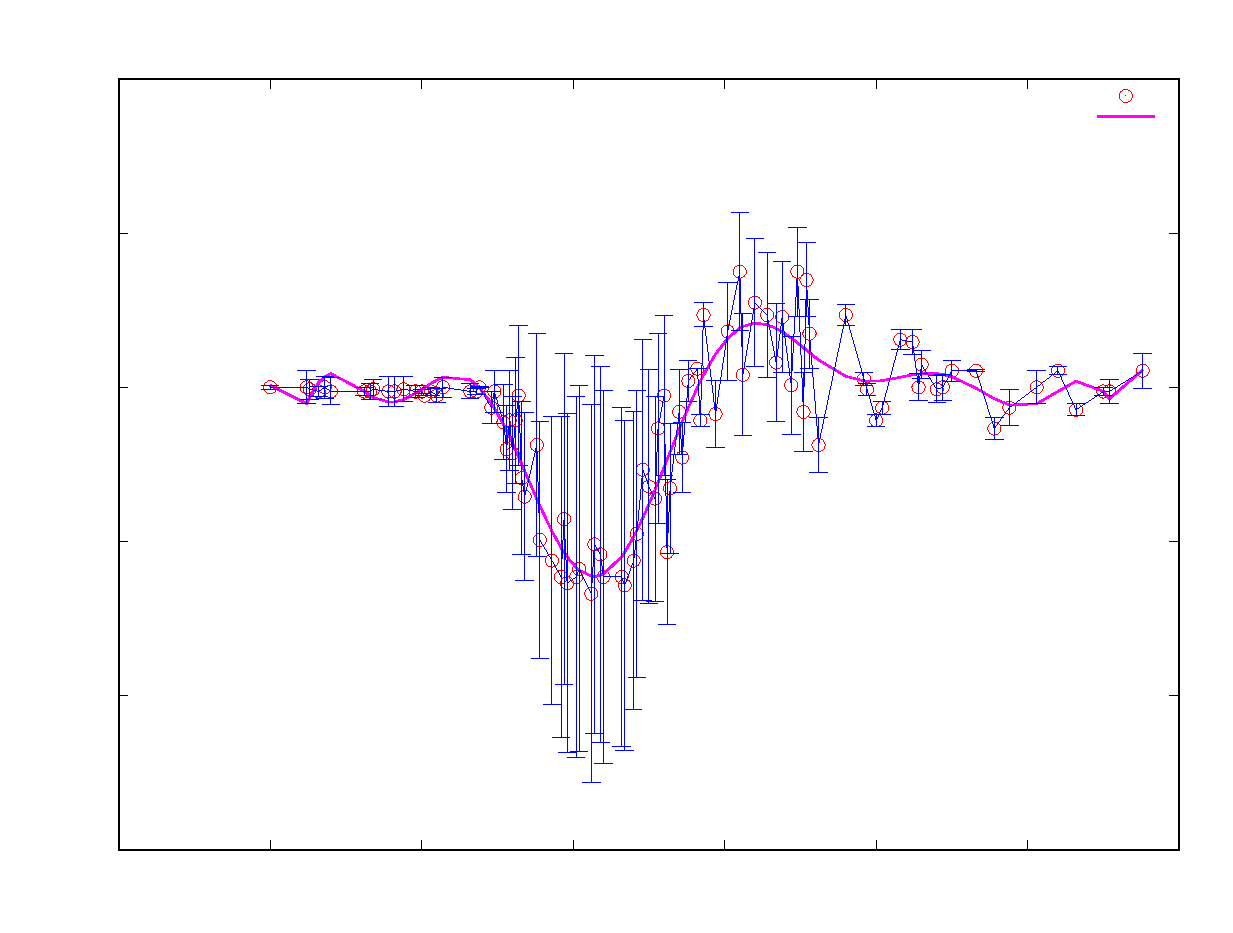
\includegraphics{poly}}%
    \gplfronttext
  \end{picture}%
\endgroup
}}
  \caption{Warmup: Polynomial Basis $n^{12}$}
\end{figure}

\subsection*{Bayesian Linear Regression}

Using Gaussian Likelihood and Prior, we solved for $W$ using Moore Penrose.
\begin{equation}
W_{ML} = (\Phi^T\Phi)^{-1}\Phi^Tt
\end{equation}

This was simple to implement, especially in Octave/Matlab. However, without normalization the error rate was close to the baseline linear basis and significantly worse than the polynomial.

\begin{figure}[h!] 
  \centering
  \scalebox{0.5}{{\large % GNUPLOT: LaTeX picture with Postscript
\begingroup
  \makeatletter
  \providecommand\color[2][]{%
    \GenericError{(gnuplot) \space\space\space\@spaces}{%
      Package color not loaded in conjunction with
      terminal option `colourtext'%
    }{See the gnuplot documentation for explanation.%
    }{Either use 'blacktext' in gnuplot or load the package
      color.sty in LaTeX.}%
    \renewcommand\color[2][]{}%
  }%
  \providecommand\includegraphics[2][]{%
    \GenericError{(gnuplot) \space\space\space\@spaces}{%
      Package graphicx or graphics not loaded%
    }{See the gnuplot documentation for explanation.%
    }{The gnuplot epslatex terminal needs graphicx.sty or graphics.sty.}%
    \renewcommand\includegraphics[2][]{}%
  }%
  \providecommand\rotatebox[2]{#2}%
  \@ifundefined{ifGPcolor}{%
    \newif\ifGPcolor
    \GPcolorfalse
  }{}%
  \@ifundefined{ifGPblacktext}{%
    \newif\ifGPblacktext
    \GPblacktexttrue
  }{}%
  % define a \g@addto@macro without @ in the name:
  \let\gplgaddtomacro\g@addto@macro
  % define empty templates for all commands taking text:
  \gdef\gplbacktext{}%
  \gdef\gplfronttext{}%
  \makeatother
  \ifGPblacktext
    % no textcolor at all
    \def\colorrgb#1{}%
    \def\colorgray#1{}%
  \else
    % gray or color?
    \ifGPcolor
      \def\colorrgb#1{\color[rgb]{#1}}%
      \def\colorgray#1{\color[gray]{#1}}%
      \expandafter\def\csname LTw\endcsname{\color{white}}%
      \expandafter\def\csname LTb\endcsname{\color{black}}%
      \expandafter\def\csname LTa\endcsname{\color{black}}%
      \expandafter\def\csname LT0\endcsname{\color[rgb]{1,0,0}}%
      \expandafter\def\csname LT1\endcsname{\color[rgb]{0,1,0}}%
      \expandafter\def\csname LT2\endcsname{\color[rgb]{0,0,1}}%
      \expandafter\def\csname LT3\endcsname{\color[rgb]{1,0,1}}%
      \expandafter\def\csname LT4\endcsname{\color[rgb]{0,1,1}}%
      \expandafter\def\csname LT5\endcsname{\color[rgb]{1,1,0}}%
      \expandafter\def\csname LT6\endcsname{\color[rgb]{0,0,0}}%
      \expandafter\def\csname LT7\endcsname{\color[rgb]{1,0.3,0}}%
      \expandafter\def\csname LT8\endcsname{\color[rgb]{0.5,0.5,0.5}}%
    \else
      % gray
      \def\colorrgb#1{\color{black}}%
      \def\colorgray#1{\color[gray]{#1}}%
      \expandafter\def\csname LTw\endcsname{\color{white}}%
      \expandafter\def\csname LTb\endcsname{\color{black}}%
      \expandafter\def\csname LTa\endcsname{\color{black}}%
      \expandafter\def\csname LT0\endcsname{\color{black}}%
      \expandafter\def\csname LT1\endcsname{\color{black}}%
      \expandafter\def\csname LT2\endcsname{\color{black}}%
      \expandafter\def\csname LT3\endcsname{\color{black}}%
      \expandafter\def\csname LT4\endcsname{\color{black}}%
      \expandafter\def\csname LT5\endcsname{\color{black}}%
      \expandafter\def\csname LT6\endcsname{\color{black}}%
      \expandafter\def\csname LT7\endcsname{\color{black}}%
      \expandafter\def\csname LT8\endcsname{\color{black}}%
    \fi
  \fi
  \setlength{\unitlength}{0.0500bp}%
  \begin{picture}(11520.00,8640.00)%
    \gplgaddtomacro\gplbacktext{%
      \colorrgb{0.00,0.00,0.00}%
      \put(860,640){\makebox(0,0)[r]{\strut{}-200}}%
      \colorrgb{0.00,0.00,0.00}%
      \put(860,1873){\makebox(0,0)[r]{\strut{}-150}}%
      \colorrgb{0.00,0.00,0.00}%
      \put(860,3106){\makebox(0,0)[r]{\strut{}-100}}%
      \colorrgb{0.00,0.00,0.00}%
      \put(860,4340){\makebox(0,0)[r]{\strut{}-50}}%
      \colorrgb{0.00,0.00,0.00}%
      \put(860,5573){\makebox(0,0)[r]{\strut{}0}}%
      \colorrgb{0.00,0.00,0.00}%
      \put(860,6806){\makebox(0,0)[r]{\strut{}50}}%
      \colorrgb{0.00,0.00,0.00}%
      \put(860,8039){\makebox(0,0)[r]{\strut{}100}}%
      \colorrgb{0.00,0.00,0.00}%
      \put(980,440){\makebox(0,0){\strut{}-10}}%
      \colorrgb{0.00,0.00,0.00}%
      \put(2434,440){\makebox(0,0){\strut{}0}}%
      \colorrgb{0.00,0.00,0.00}%
      \put(3888,440){\makebox(0,0){\strut{}10}}%
      \colorrgb{0.00,0.00,0.00}%
      \put(5342,440){\makebox(0,0){\strut{}20}}%
      \colorrgb{0.00,0.00,0.00}%
      \put(6797,440){\makebox(0,0){\strut{}30}}%
      \colorrgb{0.00,0.00,0.00}%
      \put(8251,440){\makebox(0,0){\strut{}40}}%
      \colorrgb{0.00,0.00,0.00}%
      \put(9705,440){\makebox(0,0){\strut{}50}}%
      \colorrgb{0.00,0.00,0.00}%
      \put(11159,440){\makebox(0,0){\strut{}60}}%
      \colorrgb{0.00,0.00,0.00}%
      \put(160,4339){\rotatebox{90}{\makebox(0,0){\strut{}force on head (g)}}}%
      \colorrgb{0.00,0.00,0.00}%
      \put(6069,140){\makebox(0,0){\strut{}time since impact(ms)}}%
      \csname LTb\endcsname%
      \put(6069,8339){\makebox(0,0){\strut{}Gaussian / Moore Penrose}}%
    }%
    \gplgaddtomacro\gplfronttext{%
      \csname LTb\endcsname%
      \put(10256,7876){\makebox(0,0)[r]{\strut{}Training Data}}%
      \csname LTb\endcsname%
      \put(10256,7676){\makebox(0,0)[r]{\strut{}Gaussian / Moore Penrose}}%
    }%
    \gplbacktext
    \put(0,0){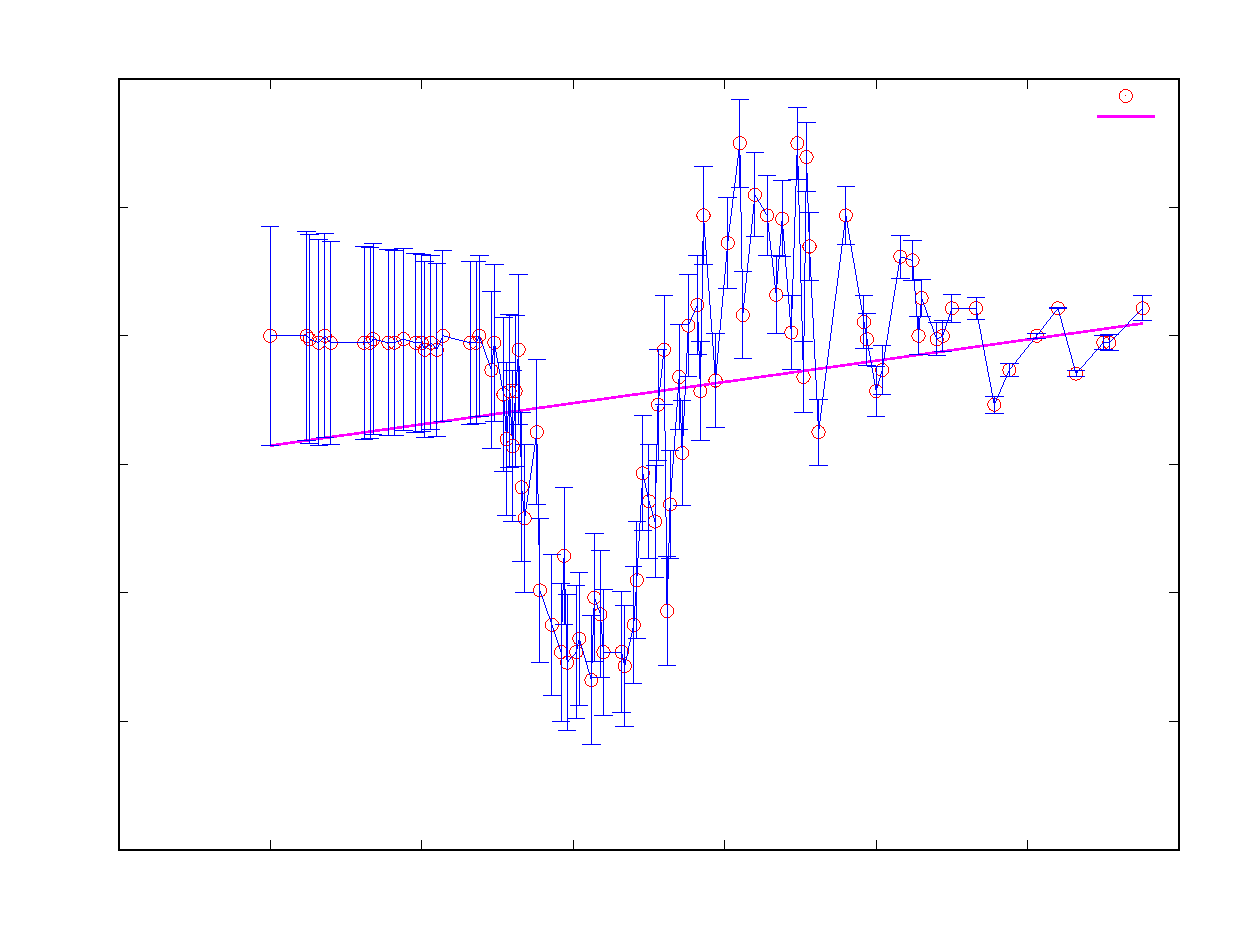
\includegraphics{gauss}}%
    \gplfronttext
  \end{picture}%
\endgroup
}}
  \caption{Warmup: Gaussian}
\end{figure}


\subsection*{Locally Weighted Linear Regression}

Locally Weighted Linear Regression (LWLR)\footnote{\emph{Machine Learning in Action} by Peter Harrington. \textsuperscript{\textcopyright} 2012 ISBN 978-1617290183} provided the lowest cost overall and a smooth fit to the data without overfitting given the profile of this dataset. A variety of $K$ values were attempted. 0.001 never converged. Values from 0.5, 1.0, 5.0 and 10.0 did converge with 1.0 seemingly providing the best balance between fit and smoothness.

LWLR is an expensive operation. Since the dataset here was small and did not match a typical straight line or polynomial pattern, it was appropriate to attempt LWLR.





\begin{figure}[h!] 
\centering
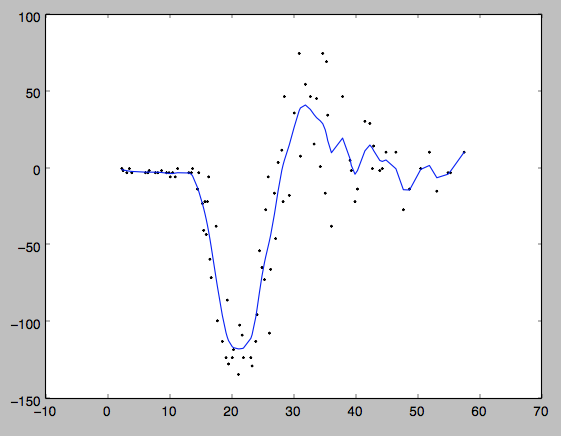
\includegraphics[scale=0.6]{lwlr}
\caption{Warmup: Locally Weighted Linear Regression $K=1$}
\end{figure}

\subsection*{Warmup Summary}
Across all basis functions, overall error rate was calculated by sum-of-squares:
\begin{equation}
J = \frac{1}{2N}\sum_{i=1}^N(y_i-t_i)^2
\end{equation}

The following table summarizes our results. LWLR was reasonably simple to implement and provided the lowest cost. For this particular dataset, it would be our basis function of choice.

\begin{center}
    \begin{tabular}{| l | l |}
    \hline
    Basis & Lowest Error \\ \hline
    Linear Basis & \hfill 1293.0 \\
    Gaussian Basis & \hfill 1187.7 \\
    Polynomial Basis & \hfill 211.9 \\
    LWLR Basis & \hfill 185.6 \\
    \hline
    \end{tabular}
\end{center}
\clearpage

\section*{Predicting Movie Opening Weekend Revenues}


\subsection*{Preliminary Data Analysis}

The training set consists of movie metadata and textual movie reviews. From the sample code provided in the problem, the initial set of features has a classic $P > N$ problem of too many dimensions (105403) for too little data (1147).  This is mostly due to the unigrams converting each word of each movie review and description into a different dimension.

Eliminating the unigrams as a first step significantly improved classification results and reduced dimensionality to only(!) 11276 dimensions. 
\subsection*{Using Cross-validation}

To quickly evaluate the regression algorithms, we built a simple cross validation set, using 10\% of the data and ten folds. This enabled us to track $J_{cv}$ vs $J_{train}$. By measuring the learning curve,\footnote{\emph{The Elements of Statistical Learning} by Hastie, et al. \textsuperscript{\textcopyright} 2009 ISBN 978-0-387848587} we could see our algorithms' progression.

Using multiple test runs, examining error rates and looking at the resulting weighting values, we were able to see which dimensions had value.



\section*{Approaches considered}
We considered two approaches: 


\subsection*{Feature Engineering}
We tested a number of approaches to both add features, and to remove features which could lead to overfitting

(1) Exclusion of unigrams.  Highly dimensional unigrams hurt model performance.

(2) Further reduction in dimensionality by examination of generated weights. For example, in the original sample code, every date (including year) was a new feature. We transformed this into month of the year, but there was no change in weighting or error rates. So this feature was eliminated.

(3) Testing of positive and negative wording in reviews. We recognized that while all words in a review may cause overfitting and result in statistically insignificant weight for an individual word (due to the small N in the data), some words in reviews could contain particularly high information content. As such, we tested two features:
\begin{description}
  \item[a `good' list]: [``good'', ``great", ``excellent", ``seeing", ``superb", ``must-see", ``fantastic", ``credible", ``best"]
  \item[a `bad' list]: [``bad", ``slow", ``boring", ``horrible", ``waste", ``poor", ``lazy",``worst"]
\end{description}
Unfortunately, that didn't improve our model's performance.

(4) Creation of squared values for all quantitative variables. This did not help model performance but did lead us to understand that the ``number of screens'' a movie was shown on was quite predictive. We then tuned the parameter for the exponent of ``number of screens'' (from 2.0 to 5.0) and found 4.3 to maximize our performance on two holdout samples -- this helped our performance gains in the model significantly.

(5) Creation of logs for all quantitative variables on the basis that large numbers (e.g. budgets) may have non-linear impacts on the revenues of a movie. This did not help the model's performance.

(6) Threshold values as binary 1/0 values for if a film's budget was above a particular value, and if the number of theaters a movie shown in was above a particular value. We ran sensitivities to various values on the logic that there can be 'step functions' insofar as a movie with a very low budget may not be sufficiently high quality, but anything about X may be sufficient). This did not help the model's performance.

By examining weighting values, error values including outliers, cross-validation rates, we concluded that only two dimensions had any significant value: \emph{number of screens} and, to a lesser extent, \emph{production budget}.


\begin{figure}[h!] 
\centering
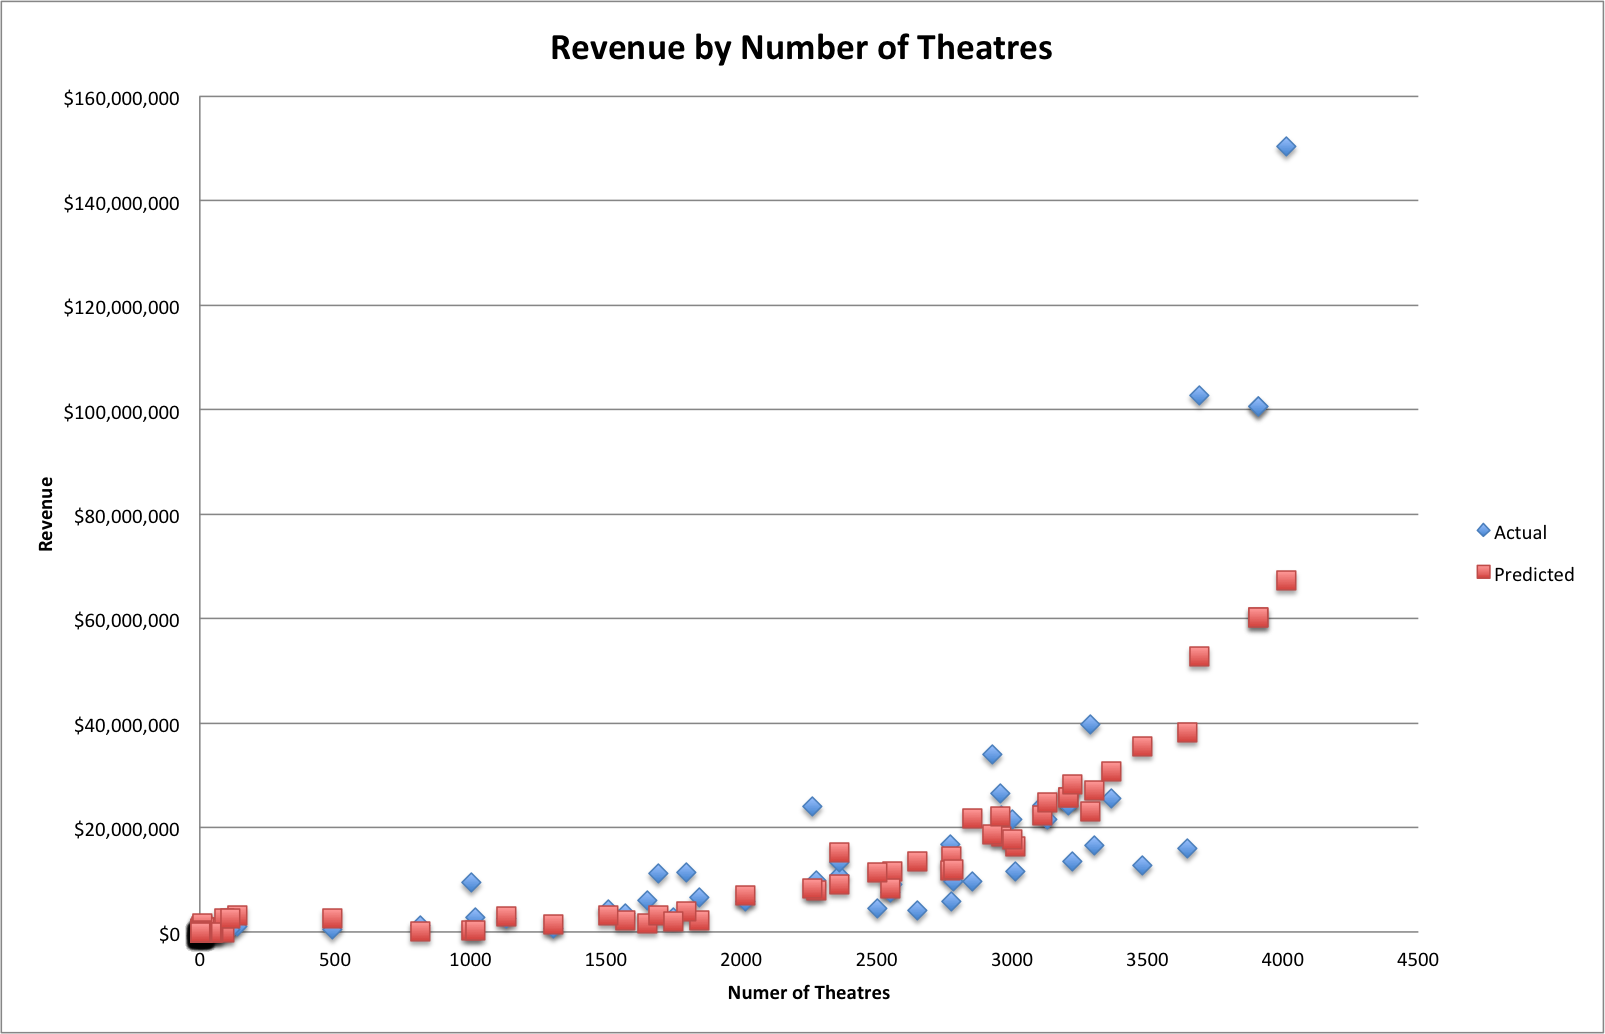
\includegraphics[scale=0.55]{numberOfTheatres}
\caption{Actual vs Predicted by Number of Screens}
\end{figure}


\subsection*{Selection of fitting technique}

We evaluated (1) ordinary least squares linear regression, (2) lasso regression (which penalizes the absolute value of regression coefficients), and (3) ridge regression (which penalizes the size of the regression coefficients). Lasso and ridge were considered to help with variable selection issues, which occur with an extremely large set of potential variables for inclusion, as was the case with unigrams.

\subsection*{Exploratory Data Analysis}

By Feature Engineering, we were able to pare the dataset down to a very manageable $1146 \times 2$, well within the bounds of a simple tool like Excel.

The largest errors were on the most successful movies. Production budgets $>$ {\$50,000,000} were deemed a "blockbuster" type. Upon detailed analysis of the training data, we needed to apply a correction of 0.85 to this different category of movie. Given the large production budget, a studio can produce only a few blockbusters per year, so by definition they are outliers compared to the majority of the movies. While our correction for large budget films decreased the overall error rate somewhat, it did not have as dramatic of an effect as we'd hoped. Given most of the big budget films had lower openings relative to smaller budget films, we assume the studios were generally also disappointed.

\section*{Conclusion}
The key learning from this practical is that even relatively simple techniques (such as linear regression) can be extremely powerful if appropriate features are selected. 

\emph{Feature Engineering} ended up being key to getting reasonable results from the linear regression. For instance, introducing polynomials of numeric information was important to capturing trends in the data. We also had to grapple with how to avoid overfitting (alas, unigrams on such a small training dataset led to significant over-fitting and had poor-out-of-sample performance), and how to represent text in a meaningful way quantitatively (something which , despite trying NLTK and `good' / `bad' lists for the text of reviews, we never quite got much signal from).

We found that what we excluded was just as important as the features we included. Poor features radically overfit and gave poor out-of-sample performance. Poor features also lacked a reasonable interpretation (e.g. what does the count of the non-stopword unigrams in a movie review really mean?). Another key learning was that more sophisticated algorithms like ridge and lasso are not necessarily better as they involve tweaking normalizing values.

Interestingly, Feature Engineering consequently required us to be more thoughtful about the problem as we sought other ways to get signal from our data. 


\end{document}  
